% Options for packages loaded elsewhere
\PassOptionsToPackage{unicode}{hyperref}
\PassOptionsToPackage{hyphens}{url}
%
\documentclass[
]{article}
\usepackage{lmodern}
\usepackage{amssymb,amsmath}
\usepackage{ifxetex,ifluatex}
\ifnum 0\ifxetex 1\fi\ifluatex 1\fi=0 % if pdftex
  \usepackage[T1]{fontenc}
  \usepackage[utf8]{inputenc}
  \usepackage{textcomp} % provide euro and other symbols
\else % if luatex or xetex
  \usepackage{unicode-math}
  \defaultfontfeatures{Scale=MatchLowercase}
  \defaultfontfeatures[\rmfamily]{Ligatures=TeX,Scale=1}
\fi
% Use upquote if available, for straight quotes in verbatim environments
\IfFileExists{upquote.sty}{\usepackage{upquote}}{}
\IfFileExists{microtype.sty}{% use microtype if available
  \usepackage[]{microtype}
  \UseMicrotypeSet[protrusion]{basicmath} % disable protrusion for tt fonts
}{}
\makeatletter
\@ifundefined{KOMAClassName}{% if non-KOMA class
  \IfFileExists{parskip.sty}{%
    \usepackage{parskip}
  }{% else
    \setlength{\parindent}{0pt}
    \setlength{\parskip}{6pt plus 2pt minus 1pt}}
}{% if KOMA class
  \KOMAoptions{parskip=half}}
\makeatother
\usepackage{xcolor}
\IfFileExists{xurl.sty}{\usepackage{xurl}}{} % add URL line breaks if available
\IfFileExists{bookmark.sty}{\usepackage{bookmark}}{\usepackage{hyperref}}
\hypersetup{
  pdftitle={Laboratório de Estatística I},
  pdfauthor={Turma MAT02031 - C},
  hidelinks,
  pdfcreator={LaTeX via pandoc}}
\urlstyle{same} % disable monospaced font for URLs
\usepackage[margin=1in]{geometry}
\usepackage{graphicx,grffile}
\makeatletter
\def\maxwidth{\ifdim\Gin@nat@width>\linewidth\linewidth\else\Gin@nat@width\fi}
\def\maxheight{\ifdim\Gin@nat@height>\textheight\textheight\else\Gin@nat@height\fi}
\makeatother
% Scale images if necessary, so that they will not overflow the page
% margins by default, and it is still possible to overwrite the defaults
% using explicit options in \includegraphics[width, height, ...]{}
\setkeys{Gin}{width=\maxwidth,height=\maxheight,keepaspectratio}
% Set default figure placement to htbp
\makeatletter
\def\fps@figure{htbp}
\makeatother
\setlength{\emergencystretch}{3em} % prevent overfull lines
\providecommand{\tightlist}{%
  \setlength{\itemsep}{0pt}\setlength{\parskip}{0pt}}
\setcounter{secnumdepth}{-\maxdimen} % remove section numbering

\title{Laboratório de Estatística I}
\author{Turma MAT02031 - C}
\date{9/3/2020}

\begin{document}
\maketitle

\begin{center}\rule{0.5\linewidth}{0.5pt}\end{center}

\hypertarget{relatuxf3rio-de-consultoria-ian---doutorando-iph}{%
\subsection{Relatório de Consultoria Ian - Doutorando
IPH}\label{relatuxf3rio-de-consultoria-ian---doutorando-iph}}

\hypertarget{objetivos-da-pesquisa}{%
\subsubsection{Objetivos da Pesquisa}\label{objetivos-da-pesquisa}}

\hypertarget{objetivos-principais}{%
\subparagraph{Objetivos Principais:}\label{objetivos-principais}}

\begin{enumerate}
\def\labelenumi{\alph{enumi})}
\tightlist
\item
  Avaliar a remoção de carbendazim por carvão ativado de casca de côco e
  biofiltração, através de ensaios de bancada e de filtros em escala
  laboratorial.
\end{enumerate}

\hypertarget{objetivos-secunduxe1rios}{%
\subparagraph{Objetivos Secundários:}\label{objetivos-secunduxe1rios}}

\begin{enumerate}
\def\labelenumi{\alph{enumi})}
\tightlist
\item
  Determinar os parâmetros da cinética de adsorção do carbendazim no
  carvão ativado granular de casca de côco a ser utilizado através de
  ensaios de bancada;
\item
  Identificação da isoterma que melhor representa a adsorção do composto
  em escala de bancada;
\item
  Identificar parâmetros operacionais como os tempos de ruptura e de
  saturação da coluna de adsorção, o Tempo de Contato de Leito Vazio
  (TCLV) e a Taxa de Aplicação Superficial (TAS), em escala
  laboratorial, para o carbendazim em água deionizada e em amostra
  efluente de decantador da Estação de Tratamento de Água Moinhos de
  Vento do Departamento Municipal de Água e Esgotos de Porto Alegre
  (DMAE);
\item
  Verificar se há competição pelos sítios de adsorção do carvão ativado
  entre o CBZ e as substâncias presentes na amostra de água da ETA;
\item
  Identificação do tempo de aclimatação para o crescimento do biofilme
  nos filtros em escala laboratorial;
\item
  Acompanhar o crescimento do biofilme bacteriano durante a realização
  dos experimentos nos filtros de areia + CAG e nos filtros
  \emph{Sandwich} em escala laboratorial;
\item
  Identificar os microorganismos presentes nos filtros de areia + CAG e
  \emph{Sandwich} em etapas diferentes dos experimentos e correlacionar
  com as variáveis analisadas;
\item
  Verificar o impacto da presença dos contaminantes emergentes no
  biofilme;
\item
  Verificar a eficiência de filtros \emph{Sandwich} e filtros de areia +
  CAG na remoção de CBZ e nos demais parâmetros de potabilidade
  dispostos na Portaria de Consolidação nº 5/2017 em escala
  laboratorial;
\item
  Verificar se a remoção biológica prolonga o tempo de vida útil do
  carvão ativado;
\item
  Verificar a eficiência dos filtros de areia + CAG e \emph{Sandwich} na
  remoção de CBZ e demais parâmetros de potabilidade da Portaria de
  Consolidação nº 5/2017 em escala piloto;
\item
  Comparar o efluente dos filtros analisados com o efluente dos filtros
  presentes na ETA.
\end{enumerate}

\hypertarget{plano-de-trabalho}{%
\subsubsection{Plano de Trabalho}\label{plano-de-trabalho}}

O estudo será divido em duas etapas:

\begin{enumerate}
\def\labelenumi{\alph{enumi})}
\tightlist
\item
  \textbf{Teste de bancada}: ocorre em menor escala e serve como etapa
  de calibragem e validação para que o experimento possa se estender
  para maior escala. O objetivo é identificar a afinidade do Carbendazim
  com o carvão ativado utilizado através dos parâmetros de cinética de
  adsorção. É utilizado um filtro composto de areia e carvão ativado
  para avaliar a absorbância do agrotóxico carbendazim em amostras de
  água pura e em amostras de água da ETA-DMAE.\\
  A abordagem em escala de bancada é a seguinte:
\end{enumerate}

\begin{enumerate}
\def\labelenumi{\arabic{enumi}.}
\tightlist
\item
  Preparação Carvão ativado

  \begin{itemize}
  \tightlist
  \item
    Transformação de carvão granular para pulverizado.
  \end{itemize}
\item
  Ensaio com agitadores 1

  \begin{itemize}
  \tightlist
  \item
    Concentração conhecida de CBZ;
  \item
    Concentração conhecida de CAP;
  \item
    Identificação do melhor tempo de contato.
  \end{itemize}
\item
  Ensaio com agitadores 2

  \begin{itemize}
  \tightlist
  \item
    Concentração conhecida de CBZ;
  \item
    Tempo de contato conhecido;
  \item
    Variação da concentração de CAP;
  \item
    Identificação da Isoterma que melhor representa o processo de
    adsorção.
  \end{itemize}
\item
  Ensaios em coluna de leito fixo

  \begin{itemize}
  \tightlist
  \item
    Concentração inicial conhecida de CBZ;
  \item
    Dimensionamento da coluna;
  \item
    Identificação dos parâmetros operacionais para coluna em escala
    real.
  \end{itemize}
\end{enumerate}

A coleta por sua vez, tem a seguinte forma:

\begin{itemize}
\tightlist
\item
  As medidas serão coletadas de 3 a 4 vezes por semana, durante 4 a 5
  meses;
\item
  Nos dias de coleta ambas efluentes serão passadas pelo filtro a cada
  15 minutos;
\item
  Será medido o pH, temperatura e absorbância percentual de agrotóxico
  na água;
\item
  Quando o filtro saturar, acabam os testes do dias e é medido o tempo
  de saturação;
\item
  Se o carvão ativado não possuir boa afinidade, é testado outro carvão;
\end{itemize}

\begin{enumerate}
\def\labelenumi{\alph{enumi})}
\setcounter{enumi}{1}
\tightlist
\item
  \textbf{Teste piloto}: aplicação do teste de bancada porém em larga
  escala. Haverão alterações no sentido de agregar mais informações no
  momento de coleta de dados, além disso, serão testados dois tipos de
  filtros, um em formato `\emph{Sandwich}' e o filtro padrão com areia e
  carvão ativado. As águas tratadas serão as mesmas, sendo uma pura com
  adição de carbendazim e outra afluente da ETA-DMAE também com
  carbendazim. A frequência amostral e os parâmetros de interesse são os
  seguintes:
\end{enumerate}

\[
\begin{array}{l|l|l}
\textbf{3x por Semana}  & \textbf{1x por semana} & \textbf{A cada 6 meses}   \\ \hline
\begin{array}[c]{@{}l@{}}\text{Turbidez};\\ \text{Cor};\\ \text{p.H};\\ \text{Temperatura da água};\\\end{array} & \begin{array}[c]{@{}l@{}}\text{Absorbância Carbendazim};\\ \text{Carbono Orgânico Total};\\ \text{E.coli};\\ \text{Coliformes};\end{array} & \text{Extração de DNA e Sequenciamento}
\end{array}
\]\\
~\\
~\\
O esquema de configuração dos filtros proposto é o seguinte:

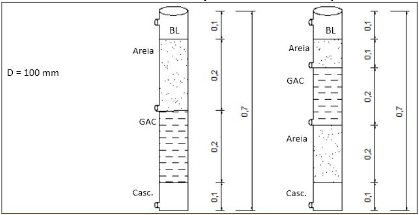
\includegraphics{/cloud/project/esquema_filtro.png}

\hypertarget{dicionuxe1rio-de-dados}{%
\subsubsection{Dicionário de Dados}\label{dicionuxe1rio-de-dados}}

\[
\begin{array}{llllllllllllll}\hline
\textbf{Nome}&& \textbf{Descrição}&& \textbf{Unid. de Medida / Escala} &\\ \hline
\text{Absorbância Carbendazim}&& \text{Capacidade de absorção da substância em seu comprimento de onda} && -log(\frac{I}{I_0}) &\\
\text{Turbidez}&& \text{Redução de transparência de um meio líquido}&& \text{NTU} &\\
\text{Cor}&& -  && \text{Unidade Hazen - uH}   &\\
\text{pH}&& \text{Indicador de acidez / basicidade em uma solução} && \text{pH}_{[0,14]} &   \\
\text{Temperatura da Água}&& - && \text{Graus Celsius  (ºC)}  &    \\
\text{Carbono Orgânico Dissolvido} && - && mg/L   &    \\
\text{Concentração E.coli}&& - && NMP/100ml      &    \\
\text{Concentração de coliformes}&& - && NMP/100ml          &\\
\text{Extração de DNA}&&-&&-&\\
\end{array}
\]\\
~\\

\hypertarget{metodologia-de-anuxe1lise-estatuxedstica-proposta}{%
\subsubsection{Metodologia de Análise Estatística
Proposta}\label{metodologia-de-anuxe1lise-estatuxedstica-proposta}}

Nesta pesquisa, estaremos fazendo uma comparação de diversos fatores
entre dois grupos distintos, buscando testar inicialmente a absorbância
do Carbendazim pelo filtro bem como o grau de influência da água impura
(com microorganismos/DMAE) em relação a água pura, sugerimos utilizar a
Análise de Variância (ANOVA).\\
Com a Análise de Variância, buscamos quantificar a variabilidade entre
grupos distintos de observações, para testar a hipótese de que as médias
entre tais grupos são significativamente iguais, desta forma, podemos
identificar qual das observações possui maior influência na variável
resposta.\\
Para facilitar o processo de análise, sugerimos que os dados sejam
tabulados de forma a listar as organizações linha a linha e as variáveis
de interesse coluna a coluna.

\end{document}
